\chapter{Controle Preditivo Baseado em Modelo}
\label{ch:mpc}

Segundo \citeonline{Rossiter2003} uma das principais diferenças entre o \acrshort{mpc} e outras
técnicas de controle (como o \acrshort{pid}, por exemplo) é que a maioria delas não leva em consideração
as ações futuras do controle, porém o \acrshort{mpc} sim, e para essas ações futuras sejam consideradas
é necessário possuir um modelo do sistema que mostre as dependências das saídas e das atuais variáveis
medidas e as entradas atuais e futuras.
Este modelo não precisa ser linear, e nem tampouco ser extremamente fiel em descrever todas as interações
físico-químicas do sistema. Na verdade, ainda segundo \citeonline{Rossiter2003}, a regra básica do modelo 
é que ele deve ser o mais simples possível, ou seja, deve ser o modelamento mínimo necessário para que
possamos observar predições com o nível de precisão necessário.

\begin{figure}[h]
    \caption{Estrutura básica do \acrshort{mpc}}
	\begin{center}
		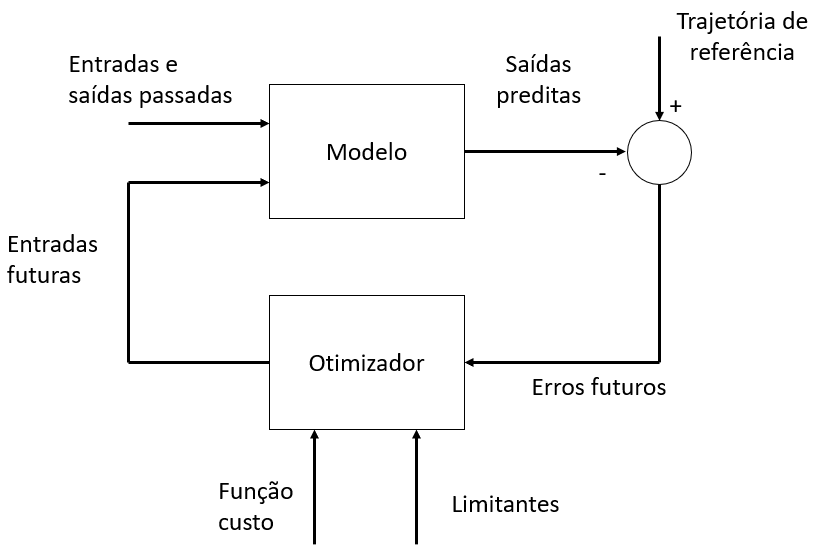
\includegraphics[width=0.75\textwidth]{./5_images/fig_mpc_basic_structure.png} 
		\label{fig:mpc_basic_structure}
    \end{center}
    \centering
    \makebox[\width]{Fonte: Autor, adaptado de \citeonline{Camacho2007}}
\end{figure}

Além de comparar com outros métodos de controle e de descrever os modelos utilizados no \acrshort{mpc},
\citeonline{Rossiter2003} também salienta alguns outros parâmetros e características que são importantes
para a técnica:

\begin{itemize}
    \item A \textbf{seleção das entradas} do sistema deve ser feita considerando a função custo que se
            deseja minimizar.

    \item O intervalo de tempo futuro, no qual o \acrshort{mpc} fará o cálculo das predições de controle
            (também conhecido como \textbf{horizonte retrocedente} (\textit{Recending Horizon}) deve
            incluir todas as dinâmicas significativas para o sistema, caso contrário o controle apresentará
            um desempenho ruim e alguns eventos não poderão ser observados.

    \item O controle será tão preciso quanto seu modelo permitir. Para conseguir um controle mais preciso
            é necessário também possuir um modelo mais preciso.

    \item Um dos principais pontos do \acrshort{mpc} é a capacidade de \textbf{lidar com restrições} on-line
            de maneira sistemática, permitindo assim uma melhor performance.

    \item Ao utilizar um modelo, este método calcula a otimização do custo levando em conta as
            \textbf{mudanças futuras na trajetória} desejada e distúrbios mensuráveis.

    \item Outra característica extremamente importante do \acrshort{mpc} é sua capacidade intrínseca de
            controlar sistemas \acrshort{mimo}.
    
\end{itemize}

% (Brincalepe) Explicar melhor este parágrafo           [removido]
% o MPC produz o sinal de controle que fornece o melhor equilíbrio entre erros de controle e mudanças
% de sinal de controle. Não é possível obter erros de controle muito pequenos e alterações de sinal de
% controle muito pequenas. Portanto, um equilíbrio sempre existirá.

% =====================================================================================================
% ============================================= Section ===============================================
% =====================================================================================================
\section{Aplicação prática}
\label{sec:aplicacao_pratica}

Segundo \citeonline{Haugen2018} tanto o \acrshort{mpc} quanto o \acrshort{mhe} são problemas praticamente
idênticos do ponto de vista matemático, pois ambos exploram um modelo matemático sobre dado um horizonte de
tempo, porém, apesar de matematicamente parecidos, eles atuam de forma inversa um ao outro, pois
enquanto o \acrshort{mhe} utiliza as variáveis de controle e os valores medidos do processo para estimar
as variáveis estados (como já apresentado na \cref{subsec:moving_horizon_estimation}), o \acrshort{mpc}
utiliza as variáveis de estado e os valores medidos do processo para estimar as variáveis de controle.
Na \cref{fig:mhe_mpc} é possível observar o \acrshort{mhe} atuando sob um horizonte de estimação, utilizando
dados passados, e o \acrshort{mpc} atuando sob um horizonte de predição, predizendo os valores futuros.

\begin{figure}
    \caption{Ação do \acrlong{mhe} e do \acrlong{mpc}}
	\begin{center}
		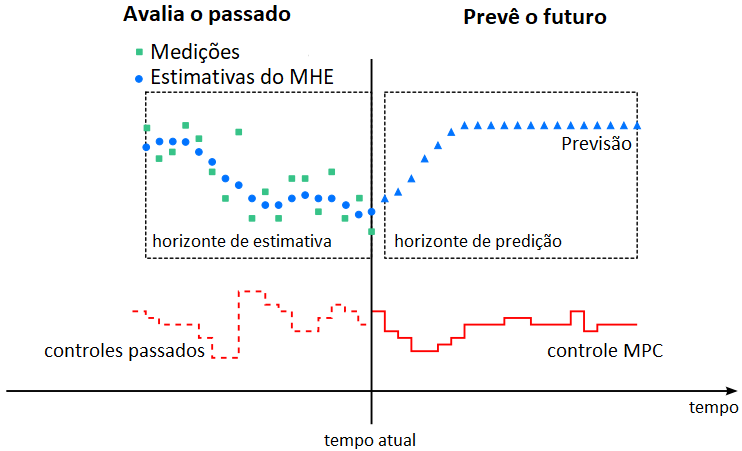
\includegraphics[width=0.9\textwidth]{./5_images/fig_mhe_mpc.png} 
		\label{fig:mhe_mpc}
	\end{center}
    \centering
    \makebox[\width]{Fonte: Autor, adaptado de \citeonline{Vukov2015a}}
\end{figure}

Podemos descrever o \acrshort{mpc} através de um problema de otimização de forma análoga ao que foi feito
na \cref{subsec:moving_horizon_estimation} para descrever o \acrshort{mhe}, porém, ao invés de minimizarmos
as variáveis de estado, devemos encontrar os valores ótimos (minimizar) das variáveis de controle.
As \crefrange{eq:mpc_minimization}{eq:mpc_minimization3} descrevem este problema de otimização.

\begin{equation}
	\label{eq:mpc_minimization}
	\min_{U} \sum_{i=k}^{k+N} ( \Vert e_i \Vert^2_{C_e} + \Vert du \Vert^2_{C_{du}} )
\end{equation}

\noindent
Onde: 
\begin{itemize}
	\item $\mathrm{U}$ é uma matriz contendo $r$ variáveis de controle nos instantes $k$ do horizonte de predição.
        \begin{equation}
            \label{eq:mpc_control_signal_matrix}
            \begin{aligned}
                \mathrm{U} &= [\mathrm{u}_{k}, \mathrm{u}_{k+1}, \cdots, \mathrm{u}_{k+(N-1)}, \mathrm{u}_N] \\
                &=
                \begin{bmatrix}
                    u(1)_{k} & u(1)_{k+1} & \cdots & u(1)_{k+(N-1)} & u(1)_N		\\
                    u(2)_{k} & u(2)_{k+1} & \cdots & u(2)_{k+(N-1)} & u(2)_N		\\
                    \vdots & \vdots & \ddots & \vdots & \vdots						\\
                    u(n)_{k} & u(n)_{k+1} & \cdots & u(n)_{k+(N-1)} & u(n)_N	
                \end{bmatrix}
            \end{aligned}
        \end{equation}
		
	\item $\mathrm{e}_i$ é o vetor de erro de controle
		\begin{equation}
			\mathrm{e}_i =
			\begin{bmatrix}
				e(1)_i \\
				e(2)_i \\
				\vdots \\
				e(m)_i \\
			\end{bmatrix}
        \end{equation}
        
        Onde $e(j)_i$ é o erro de controle da saída $j$ do processo, no instante de tempo $i$, sendo que:

        \begin{equation}
			e(j)_i = y(j)_{sp_i} - y(j)_i               
        \end{equation}
		
	\item $\mathrm{du}_i$ é o vetor de incremento da variável de controle
        \begin{equation}
            \mathrm{du}_i =
            \begin{bmatrix}
                du(1)_i \\
                du(2)_i \\
                \vdots \\
                du(r)_i \\
            \end{bmatrix}
        \end{equation}

        Onde $du(j)_i$ é o incremento da variável de controle relativo a esta mesma variável no instante
        de tempo anterior:

        \begin{equation}
			du(j)_i = u(j)_i - u(j)_{i-1}
        \end{equation}
	
	\item As matrizes $\mathrm{C_e}$ e $\mathrm{C_{du}}$ são matrizes de custo (peso) e são utilizadas
        como elementos de sintonia.

        \begin{subequations}
            \label{eq:mpc_cost_matrix}
            \begin{align}
                \mathrm{C_e} &= 
                \begin{bmatrix}
                    C_e(1,1) & \cdots & 0   		\\
                    \vdots & \ddots & \vdots		\\
                    0 & \cdots & C_e(m,m)	
                \end{bmatrix}
                                                    \\
                \mathrm{C_{du}} &= 
                \begin{bmatrix}
                    C_{du}(1,1) & \cdots & 0   		\\
                    \vdots & \ddots & \vdots		\\
                    0 & \cdots & C_{du}(r,r)	
                \end{bmatrix}
            \end{align}
        \end{subequations}
	
\end{itemize}

Substituindo as normas matriciais da \cref{eq:mpc_minimization}, temos:

\begin{equation}
    \label{eq:mpc_minimization2}
    \min_{U} \sum_{i=k}^{k+N} ( e^T_i C_e e_i + du^T_i C_{du} du_i )
\end{equation}

Expandindo então as \crefrange{eq:mpc_control_signal_matrix}{eq:mpc_cost_matrix} na \cref{eq:mpc_minimization2},
obtemos:

\begin{equation}
    \label{eq:mpc_minimization3}
    \min_{U} \sum_{i=k}^{k+N} [C_e(1,1) e(1)^2_i + \cdots + C_e(m,m) e(m)^2_i] + 
                                [C_{du}(1,1) du(1)^2_i + \cdots + C_{du}(r,r) du(r)^2_i]
\end{equation}

% .....................................................................................................
% ............................................ Subsection .............................................
% .....................................................................................................
\subsection{Exemplo}
\label{subsec:mpc_example}

O exemplo descrito nesta seção apresenta a simulação do modelo de uma planta didática de aquecimento de ar
utilizado na \textit{University College of Southeast Norway}, situada em Porsgrunn, Noruega.
Vale salientar que esta não é a planta objeto de estudo deste trabalho, sendo este apenas um exemplo
bibliográfico de aplicação de \acrshort{mpc} em planta didática, cujo modelo modelo matemático está indicado na
\cref{eq:heat_plant} e seu detalhamento construtivo pode ser melhor compreendido na \cref{fig:mpc_example_plant}.
% TODO: (Brincalepe) Detalhar melhor a planta utilizada no experimento. Acho que seria interessante detalhar a planta citada em 4.1.1
% TODO: (Brincalepe) A descrição que citei acima no item 3, pode ser feita com detalhes em 5.1. Acrescente um diagrama elétrico do sistema.
% O Brincalepe deve estar achando que a plantas do descrevendo o MPC do Haugen é a mesma do APMonitor

\begin{subequations}
    \label{eq:heat_plant}
    \begin{align}
        {\theta}_t \dot{T}_{heat} (t) &= -T_{heat} (t) + K_h [u(t - {\theta}_d) + d]     \\
        T_{out} (t) &= T_{heat} (t) + T_{env}
    \end{align}
\end{subequations}

\begin{figure}
    \caption{Planta de aquecimento de ar}
	\begin{center}
        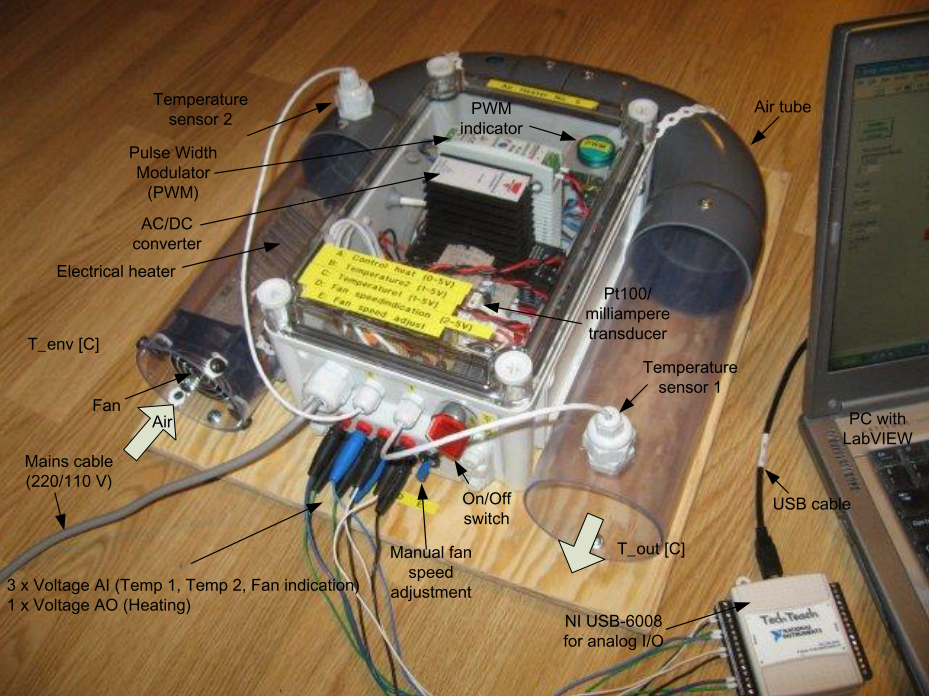
\includegraphics[width=0.9\textwidth]{./5_images/Finn_AirHeater.png} 
		\label{fig:mpc_example_plant}
	\end{center}
    \centering
    \makebox[\width]{Fonte: \citeonline{Haugen2018}}
\end{figure}

\noindent
Onde: 
\begin{itemize}
	\item $K_h$ é o ganho do aquecedor
	\item $T_{env}$ é a temperatura ambiente
	\item $T_{heat}$ é a contribuição para a temperatura total $T_{out}$ devido ao aquecedor
	\item $T_{out}$ é a temperatura do ar saindo da planta. Medido através de sensor
	\item $u$ é o sinal de controle do aquecedor
	\item $d$ é o distúrbio de entrada (adicionado ao sinal de controle)
	\item ${\theta}_d$ é o atraso que representa o transporte de ar e a dinâmica do aquecedor
	\item ${\theta}_t$ é o atraso referente à dinâmica do aquecedor
\end{itemize}

A \cref{fig:mpc_example} ilustra os dados obtidos através da execução do código-fonte \ref{lst:mpc_example},
no \cref{ch:codigos_extras}, escrito em Python.

\begin{figure}[h]
    \caption{Simulação utilizando \acrlong{mpc}}
	\begin{center}
        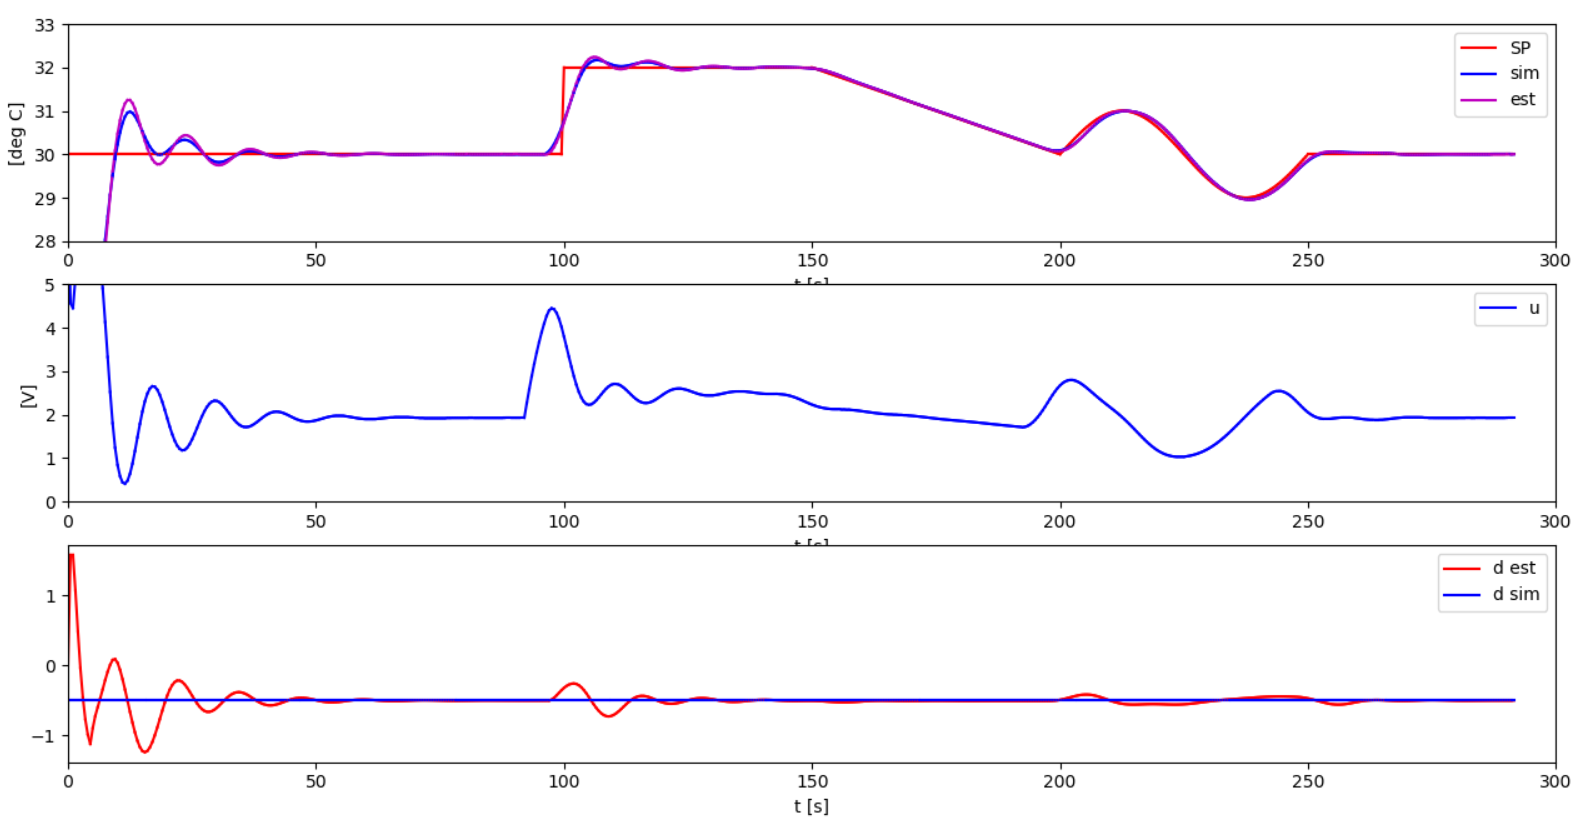
\includegraphics[width=0.9\textwidth]{./5_images/fig_mpc_example.png} 
		\label{fig:mpc_example}
	\end{center}
    \centering
    \makebox[\width]{Fonte: Autor, adaptado de \citeonline{Haugen2018}}
\end{figure}
% TODO: (Brincalepe) Interpretar imagem

% TODO: (Brincalepe) Inserir diagrama para descrever o código lst:mpc_example movido para o apendice
